\section{Motivations and Prior Work}
\label{sec:motivations}

This research began initially as an effort to demonstrate the suitability of the Rust programming language for the bioinformatics field. An exploration of the Rust-Bio project~\cite{rust} led to finding the SeqAn\footnote{SeqAn: \texttt{\url{https://www.seqan.de/}}} project for C++. Further investigation led to an understanding of the ongoing popularity of languages like Perl and Python in this area, as well. It was decided that, rather than focus specifically on Rust and its potential, this effort would instead pursue an understanding of the relative power of a selected set of languages on the metrics described.

It is believed that these three measurements can evaluate the languages with enough clarity that a programmer could make an informed choice as to which would better meet their needs.

\subsection{Programming Languages}

Programming languages have a long history. The first commercially-available compiled language was FORTRAN, first appearing in 1956. But there were languages before FORTRAN, languages that were highly specialized and often relied on obscure syntax. Languages evolve and new languages emerge as the applications of computing and the needs of software grow and expand. Some languages, such as C and later versions of Fortran, persist even as new languages intended to replace them fall out of favor and die off. When examining what makes a language successful, it is necessary to look at multiple factors:

\begin{itemize}
\item How well does it perform? How fast are the programs written in the language?
\item What aspects of problem-solving are made easier by the language? What aspects are made harder?
\item How difficult is it to develop software in the language? How difficult is it to maintain?
\end{itemize}

A comparison of languages is not only predicated on their speed but also on readability, expressiveness, and capability. A language must be able to perform, but it must also be understandable. Jokes about the relative readability and maintainability of different languages date back to the APL language if not earlier than that. Setting aside endeavors such as obfuscated code competitions, some languages are simply harder to read than their peers. Perl and Python are often compared in this regard, for example. Perl's syntax relies heavily on the use of non-alphabetic symbols (referred to as ``sigils'') in using and referencing variables. Contrast this with Python's comparatively clean syntax, which is closer in style to that of C and other similar languages.

A full treatment on the discipline of programming language design is outside the scope of this writing. Instead, issues of the more aesthetics-oriented language differences will be addressed by examining some static aspects of the code, aspects that are completely independent of the running of the programs themselves.

\subsection{Performance, Expressiveness, Energy}

The experiments that will be described in this paper were designed to focus on a trio of aspects of concern to modern software developers: how well the code performs, how easy it is to read and maintain the code, and (more recently) how the code ranks in terms of energy efficiency.

The overall performance of programs is an issue often discussed when languages are compared directly. Languages such as C and C++ offer high performance, while interpreted languages like Perl and Python have comparatively poor performance. And yet, Python holds great popularity in many sub-fields such as data science, machine learning, data visualization, and task automation. It leads to the question: why would a language so much slower would be so popular?

While there are many varied reasons why people developing software like or dislike a given language, certain aspects often rise up in conversations. These aspects include the \textit{friendliness} of the language, the \textit{ease of use} it offers, and the \textit{readability} of the language. Aspects like this are sometimes referred to as the \textit{expressiveness} of a language: the breadth of ideas that can be represented in that language, and the degree to which they can be understood and communicated.

Expressiveness can be a significant factor in language selection and use. In~\cite{berkholz}, Berkholz looks at measuring expressiveness by looking at how many lines of code change in an average version control commit for projects written in a range of languages. He found functional languages such as Lisp and Haskell to be the most expressive, and domain-specific languages to be biased towards high levels of expressiveness.

In addition to performance and expressiveness, the energy usage of software is rapidly becoming more important as data-centers try to reduce carbon footprints and developers target battery-driven mobile devices.

\begin{figure}[ht]
    \centering
    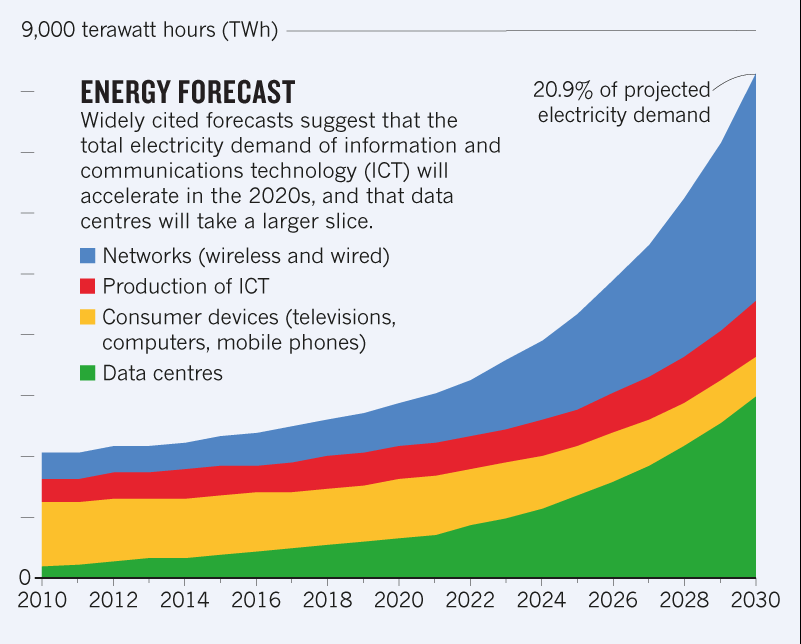
\includegraphics[width=0.85\textwidth]{figures/data-center-energy.png}
    \caption[Projected energy demands through 2030]{Projected energy demands through 2030 (original source~\cite{garcia2022})}
    \label{fig:image:energy_demands}
\end{figure}

In~\cite{garcia2022}, the author reports that the U.S. data center industry alone ``consumed around 196 to 400 terawatt-hours (TWh)'' in 2020. And as their graph above predicts, this could become significantly higher by 2030. But in~\cite{masanet} the authors point out that actual server energy use is on average only 43\% of data center usage. And yet, if accurate, this means that server energy could account for anywhere from 84 to 172 TWh. Even a small reduction in server energy could have an impact.

In~\cite{pereira}, Pereira, et al did an extensive analysis of energy efficiency at the programming language level. Upon seeing the results and the methods used, it became clear that this should be used with the previous two metrics to evaluate a set of languages in even broader terms.

\subsection{Prior Work}

Some of the papers that informed this research include:

Rahate and Chandak~\cite{rahate} performed a study focused on algorithm performance similar to what is planned here. From this paper, it was determined that there should be at least five algorithms under consideration and that algorithms such as Knuth-Morris-Pratt~\cite{knuth} would make good candidates.

In~\cite{chen2021string}, Chen and Nguyen describe an approach to string matching over DNA data with $k$ differences. Their technique was based primarily on \textit{edit distance}, and lent ideas to the development of the $k$-gap approximate-matching algorithm that will be described in~\ref{subsec:dfa_gap}.

Neamatollahi, et al~\cite{neamatollahi} describe three pattern matching algorithms that are specifically targeted at searches on large DNA sequences. While the first is a more traditional character-based matching algorithm, the second and third take advantage of aspects of the CPU such as word-width to speed up comparisons.

The concept of multiple-pattern-matching for exact matches is explored by Bhuka and Somayajulu in~\cite{bhukya}. Their approach is based on the use of pair indexing for both the sequence and the pattern. This paper gave weight to the idea of multi-pattern matching and led to the decision to take the Aho \& Corasick algorithm~\cite{aho} as one of the evaluation algorithms.

In~\cite{cheng2003approximate}, Cheng, et al describe a novel data structure and use it in two new parallel approximate matching algorithms. Ultimately, this was not used directly as the multiple-machine clusters would have greatly increased the complexity of taking energy usage measurements.

Ahmed, et al~\cite{ahmed2020efficient} presents an efficient implementation for maximal exact matching (MEM) seeds in long DNA reads, using GPU computing. While the algorithm itself appeared very sound, adding a MEM algorithm to the experiments was not practical in general. Additionally, CUDA computing was not available to all five of the chosen languages.

Xylogiannopoulos~\cite{xylogiannopoulos2019exhaustive} describes a novel methodology for exact string matching based on a pipeline of data structures and algorithms. This approach would have been beyond the scope of the goals of this paper, as the focus here is on using basic individual algorithms.

Alazzam and Sharieh~\cite{alazzam2018parallel} developed a parallel $n$-gram approach to approximate matching. As a parallel algorithm, it would not have been applicable equally across the selected languages as some (such as Python) have limitations on multi-threaded operation.
